%-------------------------------------------------------------------------------------------
\documentclass[aspectratio=169,UTF8,10pt]{ctexbeamer}

%%%%%%%%%%%%%%%%%%%%%%%%%%%%%
\usepackage{colortbl}
\usepackage{color}
\usepackage{booktabs}
\usepackage{threeparttable}
\usepackage{hyperref}
%\usepackage{babel}
%%%%%%%%%%%%%%%%%%%%%%%%%%%%%

\mode<presentation> {
\usetheme{Madrid}
%\setbeamertemplate{footline} % To remove the footer line in all slides uncomment this line
\setbeamertemplate{footline}[frame number] % To replace the footer line in all slides with a simple slide count uncomment this line
\setbeamercolor{page number in head/foot}{fg=blue}
\setbeamertemplate{navigation symbols}{} % To remove the navigation symbols from the bottom of all slides uncomment this line
}

% User Defined Block %%%%%%%%%%%%%%%%%%%%%%%%%%%%%%%%%%%%%%%%%%%%%%%%%%%%%%%%
\usepackage{setspace}
\definecolor{orange}{rgb}{1,0.5,0}
\definecolor{aa}{RGB}{34,139,34}
\definecolor{lightblue}{rgb}{0,0.85,0.9}
\definecolor{darkblue}{rgb}{0,0.7,1}
\definecolor{hanblue}{rgb}{0.27, 0.42, 0.81}
\definecolor{indiagreen}{rgb}{0.07, 0.53, 0.03}
\definecolor{indianred}{rgb}{0.8, 0.36, 0.36}
\definecolor{indianyellow}{rgb}{0.89, 0.66, 0.34}
\definecolor{babypink}{rgb}{0.96, 0.76, 0.76}
\definecolor{ao(english)}{rgb}{0.0, 0.5, 0.0}
\definecolor{bondiblue}{rgb}{0.0, 0.58, 0.71}
\definecolor{ao(english)}{rgb}{0.0, 0.5, 0.0}
\definecolor{azure(colorwheel)}{rgb}{0.0, 0.5, 1.0}
\setbeamerfont{block title}{size=\normalsize}
\setbeamerfont{block body}{size=\small}

% User Defined Block %%%%%%%%%%%%%%%%%%%%%%%%%%%%%%%%%%%%%%%%%%%%%%%%%%%%%%%%
\newenvironment<>{abstractblock}[1]{%
  \setbeamercolor{block title}{fg=white,bg=bondiblue}%
%   \setbeamercolor{block body}{fg=white,bg=bondiblue}%
  \begin{block}#2{#1}}{\end{block}}
\newenvironment<>{blueblock}[1]{%
  \setbeamercolor{block title}{fg=white,bg=hanblue}%
  \begin{block}#2{#1}}{\end{block}}

\newenvironment<>{greenblock}[1]{%
  \setstretch{1.3}\setbeamercolor{block title}{fg=white,bg=indiagreen}%
  \begin{block}#2{#1}}{\end{block}}

\newenvironment<>{redblock}[1]{%
  \setstretch{1.3}\setbeamercolor{block title}{fg=white,bg=indianred}%
  \begin{block}#2{#1}}{\end{block}}

\newenvironment<>{yellowblock}[1]{%
  \setstretch{1.3}\setbeamercolor{block title}{fg=white,bg=indianyellow}%
  \begin{block}#2{#1}}{\end{block}}

%----------------------------------------------------------------------------------------
%	PACKAGES
%----------------------------------------------------------------------------------------
\usepackage{graphicx} % Allows including images
%\usepackage{tikz}
%\usetikzlibrary{shapes.geometric, arrows}
\usepackage{listings}
\lstset{language=C++,
    columns=flexible,
   % basicstyle=\scriptsize\ttfamily,                                      % 设定代码字体、大小4
    basicstyle=\footnotesize\ttfamily,
    %numbers=left,xleftmargin=2em,framexleftmargin=2em,                   % 在左侧显示行号
    %numberstyle=\color{darkgray},                                        % 设定行号格式
    keywordstyle=\color{blue},                                            % 设定关键字格式
    commentstyle=\color{ao(english)},                                     % 设置代码注释的格式
    stringstyle=\color{brown},                                            % 设置字符串格式
    %showstringspaces=false,                                              % 控制是否显示空格
	%frame=lines,                                                         % 控制外框
    breaklines,                                                           % 控制是否折行
    postbreak=\space,                                                     % 控制折行后显示的标识字符
    breakindent=5pt,                                                      % 控制折行后缩进数量
    emph={size\_t,array,deque,list,map,queue,set,stack,vector,string,pair,tuple}, % 非内置类型
    emphstyle={\color{teal}},
    escapeinside={(*@}{@*)},
    literate={&}{{\color{red}\&}}{1}                                      %{<replace>}{<replacement text>}{<length>} no comma between items
}
%---------------------------------------------------------------------------------------------------

%%%%%%%%%%%%%%%%%%%%%%%%%%%%%%%%%%%%%%%%%%%%%%%%%%%%%%%%%%%%%%%%%%%%%%%%%%%%%%%%%%%%%%%%%%%%%%
\title[\textit{面向对象软件开发技术 }]{面向对象软件开发技术 -课程介绍}
\author[李长河]{李长河} % Your name
\institute[CUG] % Your institution as it will appear on the bottom of every slide, may be shorthand to save space
{
中国地质大学(武汉)自动化学院\\ % Your institution for the title page
\medskip
\textit{lichanghe@cug.edu.cn} % Your email address
}
\date{} % Date, can be changed to a custom date
%%%%%%%%%%%%%%%%%%%%%%%%%%%%%%%%%%%%%%%%%%%%%%%%%%%%%%%%%%%%%%%%%%%%%%%%%%%%%%%%%%%%%%%%%%%%%%

%-----------------------------------------------------------



\begin{document}

\maketitle

\begin{frame}
\begin{columns}
	\begin{column}{0.6\textwidth}
	\begin{block}{教材}
	李长河, 童恒建, 叶亚琴等, C++程序设计(基于C++11标准). \\电子工业出版社, \alert{2019年10月第3次印刷}

	\end{block}
\begin{block}{电子资源}
{\footnotesize \url{https://github.com/Changhe160/cplusplus2020-2021-1}} \\
	\end{block}
\begin{block}{参考书}
	Stanley B. Lippman,Jos\'{e}e Lajoie,Barbara E. Moo.C++ Primer(第五版).王刚等译.北京:电子工业出版社,2013.	
	\end{block}
	\end{column}
	\hfill
	\begin{column}{0.35\textwidth}
		\begin{figure}[ht]
			\centering
			
\includegraphics[scale=0.8]{book.jpg}
		\end{figure}
	\end{column}
\end{columns}
\end{frame}


%-----------------------------------------------------------
\begin{frame}
\begin{columns}
\column{0.45\textwidth}
\begin{block}{学习目标}
\begin{enumerate}
\item 掌握 {\color{red}面向对象}程序设计方法;
\item 运用常见 {\color{red}数据结构和算法}解决实际问题;
\item {\color{blue}熟悉可视化程序设计开发工具(Qt)。}
\end{enumerate}
\end{block}

\begin{block}<3->{课时安排}
讲课学时:28,实验学时:4(上机考试)
\end{block}
\column<2->{0.5\textwidth}
\begin{tabular}{cc}
  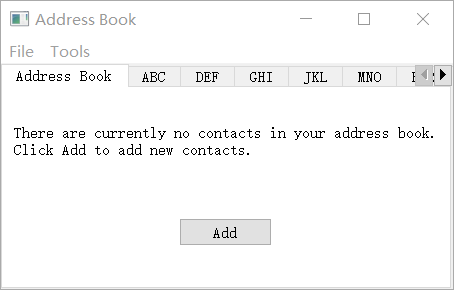
\includegraphics[scale=0.26]{addressbook.png}&
  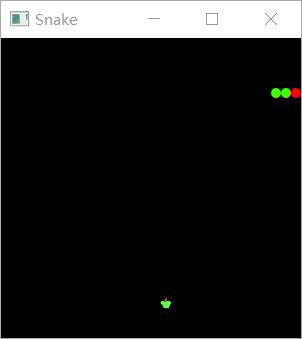
\includegraphics[scale=0.22]{snake.png}
\end{tabular}

\end{columns}


\begin{block}<4->{课程考核}
课程总成绩 = 考勤*5\%+四次上机考核*40\%+1次综合考核*40\%+ 课程报告*15\%\\
考核方式:线上提交+线上验收~~\url{http://course.educg.net/indexcs/simple.jsp?loginErr=0}
\end{block}

\end{frame}


%-----------------------------------------------------------
\begin{frame}
\begin{columns}
\column{0.45\textwidth}
\begin{block}{课程纪律}
\begin{enumerate}
\item 课上严禁看手机;
\item 上机验收严禁抄袭,一经发现,均记0分处理。
\end{enumerate}
\end{block}
\begin{block}<2->{课程群}
  QQ群:940393564\\
  助教:杨瑞
\end{block}
\column{0.45\textwidth}
\begin{center}
  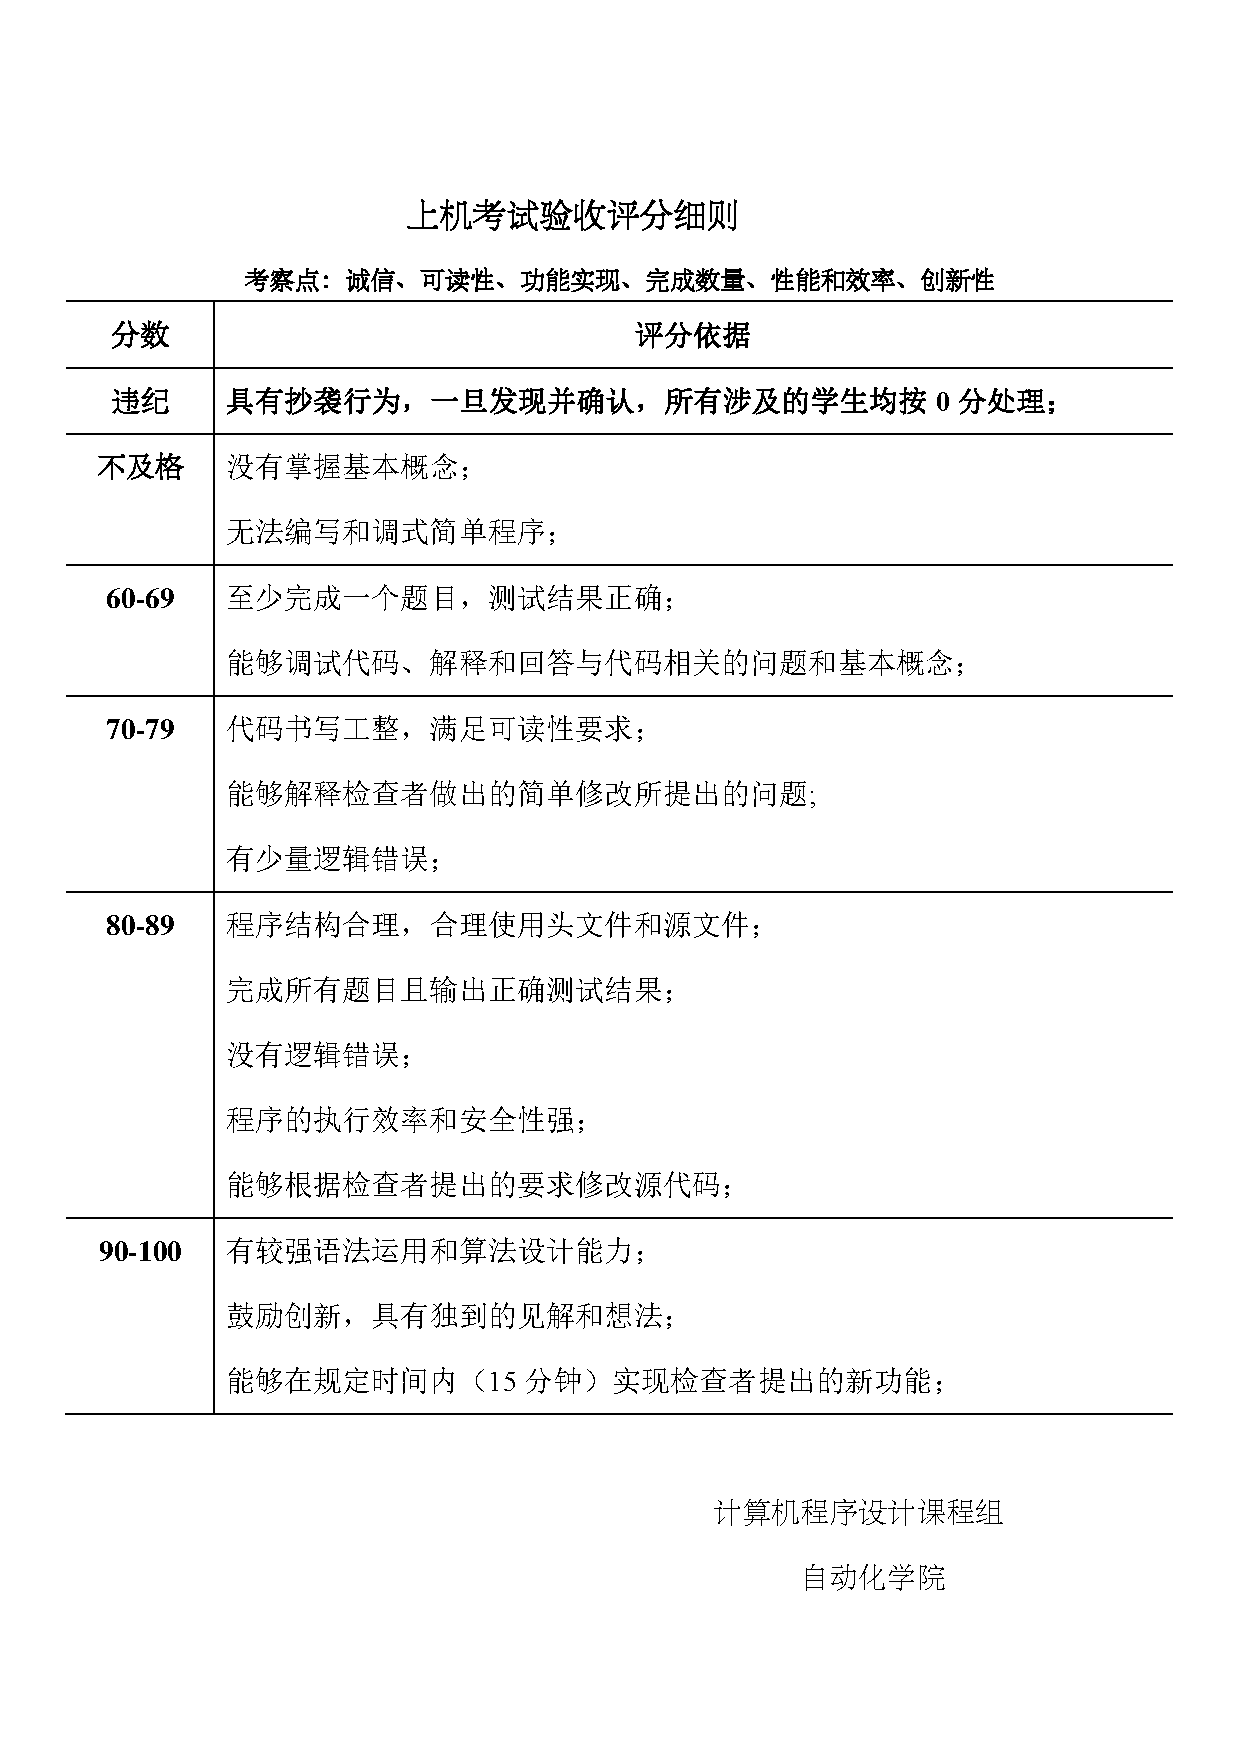
\includegraphics[scale=0.3]{上机考核评分依据.pdf}
\end{center}
\end{columns}
\end{frame}

\end{document}
